\documentclass{../res/univ-projet}

\usepackage[francais]{babel}
\usepackage{lscape}

%couleur perso
\definecolor{bleu}{RGB}{91,155,213}
\definecolor{orange}{RGB}{235,125,3}
\definecolor{vert}{RGB}{71,191,43}

\logo{../res/logo_univ.png}
\title{Plan de Développement}
\author{Olivier \bsc{Thibault}}
\projet{Projet PGP}
\projdesc{Etude et implantation d'un outil graphique de gestion de clé PGP}
\filiere{Master 1 SSI }
\matiere{Conduite de projet}
\version{0.3}
\relecteur{}
\date{Janvier 2015}

\histentry{0.1}{14/12/2014}{Vertion initiale}
\histentry{0.2}{01/01/2015}{Ajout de la partie planing}
\histentry{0.3}{07/01/2015}{Finalisation des parties 7, 8 et 9}

\begin{document}
%Page de garde
\maketitle
\newpage
%La table des matières
~
\tableofcontents
\newpage

%----------------------------------------------------------------------------------------------------------------------------------------------
\section{\underline{Contexte du projet}}

\subsection{Origine du projet}

GnuPG est un logiciel libre en ligne de commandes, qui permet de réaliser un certain nombre d'opérations cryptographiques, sur des messages ou 
documents, ainsi que de gérer un trousseau de clés. Cet outil peut paraître assez complexe à appréhender pour un utilisateur novice, 
car il existe un grand nombre de commandes et d'options différentes. 

La solution serait d'utiliser une interface graphique, qui présenterait de manière plus claire les possibilités de GnuPG. Il en existe quelques 
unes comme Kgpg, Seahorse ou Gpa, mais malheureusement, ces interfaces ne permettent pas d'exploiter pleinement GnuPG. En effet, certaintes 
commandes n'y sont pas implantées, ce qui oblige les utilisateurs à revenir en ligne commandes pour pouvoir effectuer certaines opérations. 

Le projet consistera donc, en partie, à proposer une interface répondant à ces problèmes.

\subsection{Contexte de développement}

Ce projet s'inscrit dans le cadre de la formation du master 1 en sécurité des systèmes informatiques de l'UFR des sciences et techniques de Rouen. 
La période de réalisation s'étend de fin janvier à début mai 2015. 

Il est demandé de développer ce projet de manière ``Agile''. Cela se caractérise donc par un style de conduite de projet itératif incrémental, 
centré sur l’autonomie des ressources humaines impliquées dans la spécification, la production et la validation d’une application intégrée et 
testée en continu. L'équipe en charge du projet et la cliente doivent travailler le plus possible ensemble, de manière à permettre une meilleure 
réactivité des développeurs face à l'évolution éventuelle du besoin. Il sera nécessaire de livrer fréquemment une version opérationnelle avec 
des cycles de quelques semaines, afin de s'assurer de la satisfaction de la cliente.

Des audits sont prévus en cours d'année afin de contôler la qualité de gestion du projet.

\subsection{Principaux acteurs}

Ce projet est proposé par Mme. Magali BARDET (enseignante et responsable du master SSI à l'UFR des sciences et techniques de Rouen) 
afin d'apporter une solution au problème décrit au point 1.1. La cliente pourra aussi soutenir techniquement l'équipe en charge du projet du 
fait de ses nombreuses connaissances en cryptographie.

M. Karim Abdellah GODARD est un intervenant et assure le rôle de consultant en gestion de projet.

L'équipe en charge du développement est constituée de sept étudiants actuellement en première année du master SSI de Rouen : 
\\

\begin{tabular}{ll}
- Bertille BOUILLIE & Reponsable client \\
- Guillaume LEROY & Architecte \\
- Ibrahima Sory BARRY & Chargé client \\
- Lucas BARBAY & Testeurs \\
- Matthieu FIN & Responsable technique \\
- Pierre BALMELLE & Responsable qualité \\
- Olivier THIBAULT & Chef de projet \\
\end{tabular}

\newpage

\subsection{Objectifs poursuivis}

Dans un premier temps, il est demandé de réaliser une étude complète de GnuPG ainsi que du standard sur lequel il repose (OpenPGP), en vue de 
rédiger un rapport illustrant toutes les fonctionnalités. Ce rapport doit permettre à un utilisateur novice en PGP de comprendre cet outil, 
il doit donc être rédigé dans un esprit pédagogique. De ce fait, le premier objectif est d'aquérir une connaissance pointue du sujet, tout en 
se rappelant les questions que nous nous sommes posées au fil de cette étude. Nous devrons être capable de prendre assez de recul de manière a 
pouvoir expliquer les choses comme nous l'aurions souhaité en tant que novice.

Ensuite, une interface graphique permettant d'exploiter pleinement les fonctionnalités de GnuPG de manière conviviale et pédagogique doit être 
proposée. Les technologies choisies pour la développer sont C++ et Qt5. L'objectif est donc de maîtriser au mieux ces technologies afin 
de fournir une application de qualité, qui satisfera pleinement la cliente. Le défi est aussi de faire un effort particulier quand à l'ergonomie 
et l'intuitivité de l'interface, surtout en ce qui concerne la partie toile de confiance. L'application devra être accompagnée d'un manuel 
d'utilisation et inclure une aide pour guider l'utilisateur. Ces deux points nécessiteront un certain recul sur nos travaux pour qu'ils 
puissent être parfaitement compréhensibles par un novice en PGP.

Enfin, il est demandé d'effectuer une étude des limites cryptographiques de PGP et de produire un document qui décrit ces limites. \`{A} travers 
ce document, l'objectif est de renforcer notre sens de l'analyse en tant que futur professionnel de la sécurité informatique.

\subsection{Documents de référence}

Documents utiles à l'étude du sujet: \\
\begin{itemize}
\item Définitions du standard OpenPGP \href{http://tools.ietf.org/html/rfc4880}{RFC 4880}.
\item Le manuel de GnuPG: \href{https://www.gnupg.org/documentation/manuals/gnupg/}{https://www.gnupg.org/documentation/manuals/gnupg/}.
\item Le guide utilisateur de GnuPG: \href{https://www.gnupg.org/gph/fr/manual.html}{https://www.gnupg.org/gph/fr/manual.html}.
\item Exemple de visualisation d'une toile de confiance: \href{https://www.archlinux.org/master-keys/#visualization}{https://www.archlinux.org/master-keys/\#visualization}. \\
\end{itemize}


Documents de gestion de projet: \\
\begin{itemize}
\item La spécification technique du besoin: Ce document traduit les besoins du client et recence les engagements de notre équipe dans le cadre du projet.
\item Le cahier de recette: Ce document présente les moyens mis en oeuvre afin de vérifier que le produit est conforme aux attentes du client.
\item Le document d'architecture logiciel: Ce document décrit les solutions techniques proposées et notre démarche de développement.
\item Le document d'analyse des risques: Ce document établit les risques qui pourraient nuire au bon déroulement du projet ainsi que les solutions associées.
\end{itemize}

\newpage

%---------------------------------------------------------------------------------------------------------------------------------------------
\section{\underline{Méthodologie de développement}}

Notre méthodologie de développement s'inspirera majoritairement de la méthode agile Scrum et quelque peu d'Extreme Programming en ce qui concerne les tests. 
Le projet sera donc découpé en boîtes de temps (appelées ``sprints''), de quatre semaines environ, et comportant différentes étapes : \\\\

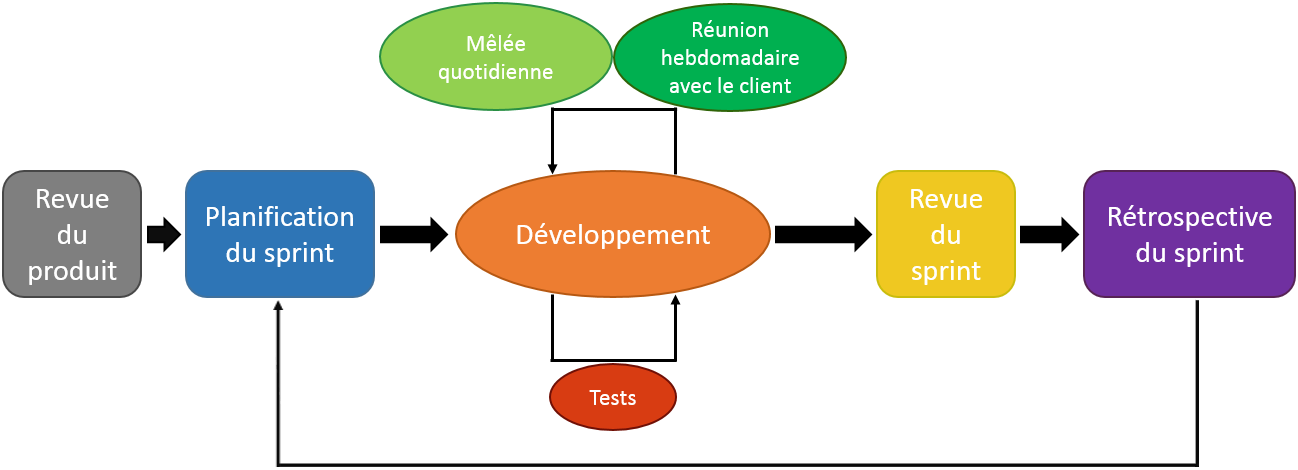
\includegraphics[scale=0.45]{./graphics/Schema_methodologie_developpement} \\
\begin{center}
 \textbf{\textit{Figure 1: Schéma d'un sprint}} \\~\\
\end{center}


\subsection{Revue du produit :} 

Cette étape a déjà été effectuée pendant la phase de l'avant projet et est materialisée par la spécification technique du besoin. Cependant, à chaque début de 
sprint, une réunion avec la cliente permettra de mettre à jour le document en fonction de l'évolution du besoin si nécessaire.

\subsection{Planification du sprint :} 

Cette étape est déjà en partie réalisé pour les sprints prévus mais sera peut-être amené à évoluer au cours du projet. C'est pourquoi, en début de sprint, 
un but est décidé en fonction de l'état d'avancement du projet. Pour atteindre cet objectif, toute l'équipe devra définir avec la cliente, lors d'une réunion de 
planification de sprint, quels éléments du carnet du produit seront réalisés. 

\subsection{Développement :} 

Cette étape est constituée de plusieurs évènements :

Avant chaque journée de développement aura lieu une réunion (la mêlée quotidienne). Cet évènement permet aux 
développeurs de faire un point de coordination sur les tâches en cours et sur les difficultés rencontrées. Cette réunion dure environ quinze minutes et ne 
concerne que l'équipe des développeurs.

Chaque semaine l'équipe se réunira avec la cliente afin de faire le point sur l'avancement, ainsi que pour échanger d'éventuelles questions ou faire part 
de changement.

Chaque composant développé devra passer des tests unitaire, d'intégration et validation. Ces tests seront écrits par les testeurs et mis à disposition des autres 
développeurs. Ils devront éventuellement être modifier ou compléter si besoin. La cliente pourra aussi demander d'effectuer ces tests lors d'une réunion afin 
de vérifier la qualité du produit.

\subsection{Revue du sprint :} 

\`{A} la fin d'un sprint, l'équipe et la cliente se réuniront pour effectuer la revue du sprint. L'objectif de la revue est de valider l'incrément de produit 
qui a été réalisé pendant le sprint. L'équipe présentera les tâches réalisées et fournira au préalable le livrable au client. Ensuite, une discussion sur 
l'état courant du projet amènera ou non à un ajustement du produit. 

\subsection{Rétrospective du sprint :} 

Cette étape se fait avec l'ensemble de l'équipe Scrum (Cliente, Scrum master et développeurs). Elle a pour but l'adaptation aux changements qui surviennent au 
cours du projet et l'amélioration continue du processus de réalisation. L'objectif est donc de relever d'après l'itération précédente, les éléments du processus 
qui ont bien fonctionnné et ceux qui sont à améliorer. Il s'en déduira un plan d'actions d'améliorations à mettre en place lors de l'itération suivante.

%---------------------------------------------------------------------------------------------------------------------------------------------
\section{\underline{Organisation et responsabilités}}

\begin{center}
 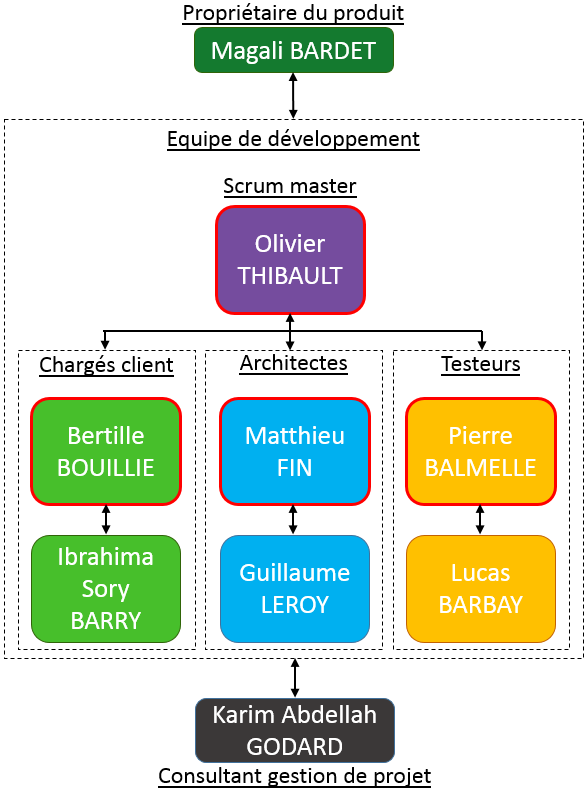
\includegraphics[scale=0.65]{./graphics/Organigramme_roles} \\~\\
 \textbf{\textit{Figure 2: Organigramme des participants au projet}}
\end{center}

\underline{Propriétaire du produit :} \\

La propriétaire du produit est la cliente mais représente aussi les utilisateurs du produit. Son rôle est de définir les éléments du produit, l'ordre dans lequel 
les fonctionnalités seronts développées et doit s'assurer que le produit est compris de l'équipe de développement. C'est également la cliente qui fixe les objectif 
d'un sprint, et peut à tout moment l'interrompre en cours.

Il est aussi important que la cliente reste disponible pour répondre aux questions de l'équipe ou pour lui faire part de ses retours. La cliente fait partie intégrante 
de l'équipe Scrum. \\

\underline{Equipe de développement :} \\

L'équipe de développement est constituée de sept personnes. Chaque membre de l'équipe possède un second rôle spécifique. L'équipe a pour résponsabilité de livrer à 
chaque fin d'itération une nouvelle version de l'application enrichie de nouvelles fonctionnalités et potentiellement utilisable. \\

\underline{Scrum master :} \\

Le Scrum master est responsable de la compréhension, de l'adhésion et de la mise en oeuvre de la méthode. C'est un ``leader au service de l'équipe''. Il assiste chaque 
rôle de l'équipe Scrum dans son activité. Il définit la durée des itérations, des modalités et de l'odre du jour des réunions.

Il a aussi d'autres attributions commes :
\begin{itemize}
 \item communiquer la vision et les objectifs à l'équipe;
 \item faciliter les rituels de Scrum ;
 \item coacher l'équipe de développement ;
 \item écarter les éléments pouvant perturber l'équipe ;
 \item aider à la coordination.
\end{itemize} ~\\

\underline{Chargés client :} \\

Les chargés clients représente l'équipe de développement auprès du client. Ils sont là pour faciliter la communication entre l'équipe et le propirétaitaire du produit. 
Ils doivent être capable d'avoir une vision à la fois général et technique du produit. Les chargés client doivent donc être en mesure de reformuler le besoin et de le 
spécifier afin d'en assurer la compréhension par l'équipe en tenant compte de l'approbation du propirétaitaire du produit. \\

\underline{Architectes :} \\

Les architectes ont pour mission de concevoir et de modéliser les différents composants de l'application à développer à partir de la spécification technique de besoin. 
C'est eux qui définissent l'environnement technique de développement (langages, outils...). Ils ont aussi un rôle de support technique si besoin pour les autres 
membres de l'équipe. \\

\underline{Testeurs :} \\

Les testeurs sont chargés de concevoir et écrire les tests permettant la validation du code de l'application. Ils sont les responsables de la qualité du produit. Leurs 
tests doit donc non seulement vérifier la validité du code et son bon fonctionnement, mais aussi la validité vis à vis des exigences du propriétaire du produit. \\
\newpage
\underline{Consultant gestion de projet :} \\

Le consultant veille à l'aquisition des connaissances nécessaires et guide l'équipe dans la succession des étapes. Il est présent pour former l'équipe et contrôler le bon 
avancement du projet, ainsi que pour répondre à d'éventuelle question des membres de l'équipe de développement. Il réalisera deux audits en cours de réalisation. \\

%---------------------------------------------------------------------------------------------------------------------------------------------
\section{\underline{Organigramme des tâches}}

Voici l'organigramme des tâches élémentaires définit pour les trois sprints prévus :

\begin{center}
 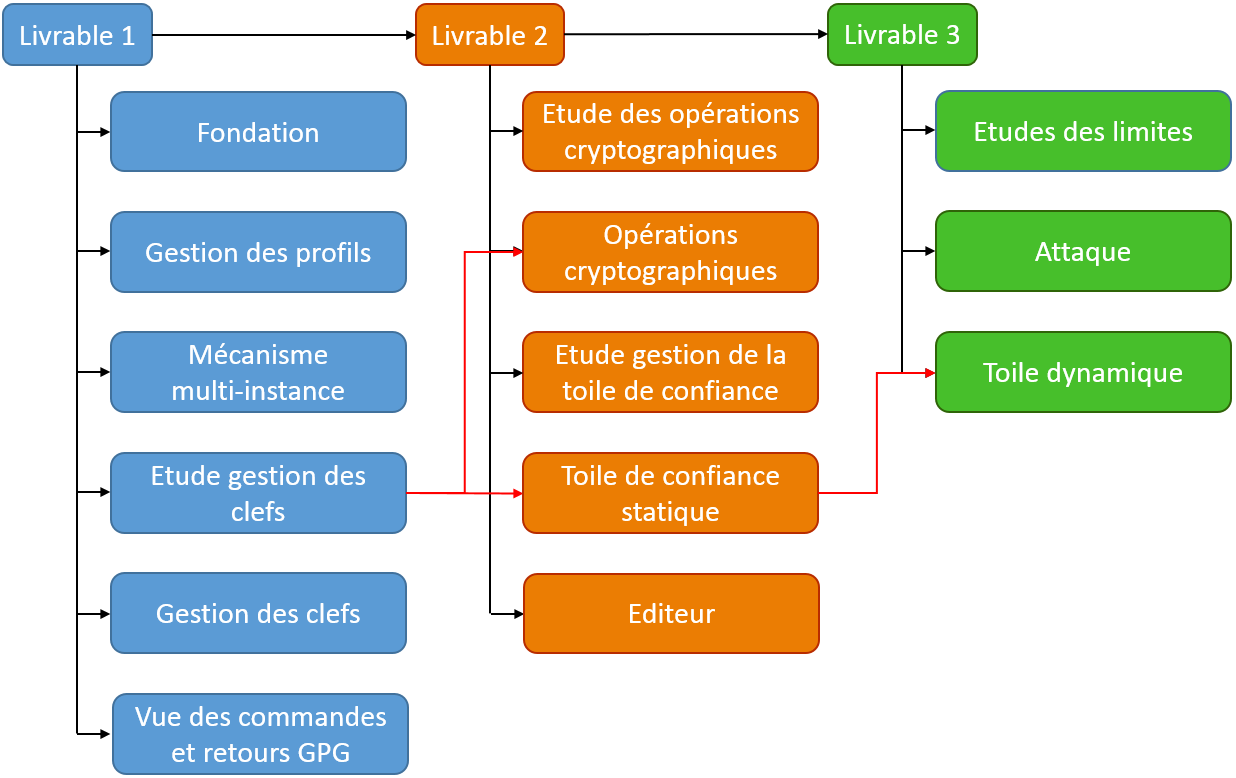
\includegraphics[scale=0.45]{./graphics/Organigramme_des_taches} \\~\\
 \textbf{\textit{Figure 3: Organigramme des tâches}}
\end{center}

\`{A} l'intérieur de ces tâches, des sous-tâches seront définies et réalisées soit par un membre soit en binôme.

Les flèches rouges indiquent une dépendance entre tâches élémentaires.
\newpage
%---------------------------------------------------------------------------------------------------------------------------------------------
\section{\underline{Évaluation du projet et dimensionnement des moyens}}
\subsection{Évaluation globale de la charge}

Le tableau ci dessous a été obtenue selon la technique d'estimation POKER. La charge exprimée en pourcent correspond donc à une moyenne des estimations de chaque membre 
de l'équipe de développement.

En bleu sont représentées les tâches du premier sprint, en orange celles du second, et en vert celles du derniers.
\begin{center}
  \begin{tabular}{|l|l|}
    \hline
    \multicolumn{1}{|c|}{\cellcolor{gray} \color{white}Catégories} & \multicolumn{1}{|c|}{\cellcolor{gray} \color{white}Charge (\%)} \\
    \hline
    \cellcolor{bleu}\color{white}Fondation & \multicolumn{1}{|c|}{\cellcolor{bleu}\color{white}5} \\
    \hline
    \cellcolor{bleu}\color{white}Mécanisme multi-instance & \multicolumn{1}{|c|}{\cellcolor{bleu}\color{white}2} \\    
    \hline
    \cellcolor{bleu}\color{white}Gestion des profils & \multicolumn{1}{|c|}{\cellcolor{bleu}\color{white}6} \\
    \hline
    \cellcolor{bleu}\color{white}\'{E}tude gestion des clefs & \multicolumn{1}{|c|}{\cellcolor{bleu}\color{white}6} \\
    \hline
    \cellcolor{bleu}\color{white}Gestion des clefs & \multicolumn{1}{|c|}{\cellcolor{bleu}\color{white}9} \\
    \hline
    \cellcolor{bleu}\color{white}Vue des commandes et retours GPG & \multicolumn{1}{|c|}{\cellcolor{bleu}\color{white}2} \\
    \hline
    \cellcolor{orange}\color{white}\'{E}tude des opérations cryptographiques & \multicolumn{1}{|c|}{\cellcolor{orange}\color{white}6} \\
    \hline
    \cellcolor{orange}\color{white}Opérations cryptographiques & \multicolumn{1}{|c|}{\cellcolor{orange}\color{white}7} \\
    \hline
    \cellcolor{orange}\color{white}\'{E}tude gestion de la toile de confiance & \multicolumn{1}{|c|}{\cellcolor{orange}\color{white}8} \\
    \hline
    \cellcolor{orange}\color{white}Toile de confiance statique & \multicolumn{1}{|c|}{\cellcolor{orange}\color{white}11} \\
    \hline
    \cellcolor{orange}\color{white}\'{E}diteur & \multicolumn{1}{|c|}{\cellcolor{orange}\color{white}4} \\
    \hline
    \cellcolor{vert}\color{white}\'{E}tude des limites & \multicolumn{1}{|c|}{\cellcolor{vert}\color{white}12} \\
    \hline
    \cellcolor{vert}\color{white}Attaque & \multicolumn{1}{|c|}{\cellcolor{vert}\color{white}12} \\
    \hline
    \cellcolor{vert}\color{white}Toile dynamique & \multicolumn{1}{|c|}{\cellcolor{vert}\color{white}10} \\
    \hline
    Total & \multicolumn{1}{|c|}{100} \\
    \hline
  \end{tabular}
\end{center}
\begin{center}
 \textbf{\textit{Figure 4: Tableau d'évaluation de la charge par tâche}}
\end{center}

Le premier sprint a donc une charge de 30\%, le second 36\%, et le dernier 34\%.

\subsection{Besoin en moyens et en ressources}

Il a été décidé que l'application sera codé en C++ et Qt5. Pour cela, chaque membre de l'équipe de développement devra installer sur son ordinateur 
QtCreator 3.3, qui est un EDI permettant de développer ce type de projet. Pour les tests, le module Qt test ainsi que le framework Cppunit seront utilisés.

Tout le contenu des livrables sera sur notre dépot Gitlab, le même que celui utilisé pour gérer les documents d'avant projet.

Pour la communication à distance, l'espace Slack utilisé lors de l'avant projet sera toujours à disposition de l'équipe.
\newpage
%---------------------------------------------------------------------------------------------------------------------------------------------

\section{\underline{Planning général}}

Entre la date de début et de fin de réalisation nous avons 16 semaine de disponible. Pour des raisons de départ prévu, des révisions et d'autres projet 
scolaire à venir, nous avons décidé de décompter les 3 semaines de vacances scolaires, ce qui nous donne 13 semaines. Une semaine de marge est prévue 
et nous ramène ainsi à 12 semaines de développement. 

Le projet sera découpé en trois sprints de 4 semaines. Une semaine comptera 5 jours de développement, du lundi au 
vendredi. Le projet comptera donc 60 jours de travail, soit 20 jours par sprint.

Nous estimons une moyenne de disponibilité par membre à une 1h30 par jour. Soit pour 7 développeurs, 52h30 de temps de travail par semaine, donc 
210h par sprint pour réaliser un certain nombre de tâches. \\

Le premier jour de chaque sprint aura lieu une réunion permettant de mettre au claire la planification de celui ci. En cours de sprint, les réunions 
hebdomadaires qui ne figure pas sur le planning devront être prévue avec le propriétaire du produit. \`{A} la fin du sprint, aura lieu la 
ou les réunion(s) de présentation du livrable, et de rétrospective. \\

\textit{Vous trouverez en annexe le planing général ainsi que celui du sprint 1.} \\

%---------------------------------------------------------------------------------------------------------------------------------------------
\section{\underline{Procédés de gestion}}
\subsection{Gestion de la documentation}

Au cours du projet plusieurs documents devrons être rédigés :
\begin{itemize}
 \item Un rapport sur l'étude de GnuPG/OpenPGP;
 \item Un rapport sur l'étude des limites de PGP;
 \item Un manuel d'utilisation de notre application.
\end{itemize} ~\\

En ce qui concerne le rapport sur l'étude de GnuPG/OpenPGP ainsi que le manuel d'utilisation, chacun aura pour résponsabilité de rédiger une partie 
du document en rapport avec les tâches qu'il aura choisi de développer. Pour l'études des limites la question n'a pas encore été réfléchie. Chacun 
des membres devra relire les parties qu'il n'a pas rédigé afin d'apporter des suggestions éventuelles. Les documents devront ensuite être approuvés 
par la cliente.

En ce qui concerne leur gestion, il seront stockés sur notre dépot Gitlab, au sein du répertoire ``documents`` et d'un sous répertoire du même nom 
que le document à produire. Ils seront rédiger en LaTeX selon la demande du propirétaitaire du produit.
\newpage
\subsection{Gestion des configurations}

Le code produit sera stockés sur notre dépot Gitlab. Voici le workflow qui sera mis en place pour gérer l'évolution et les différentes version 
produites: \\

\begin{center}
 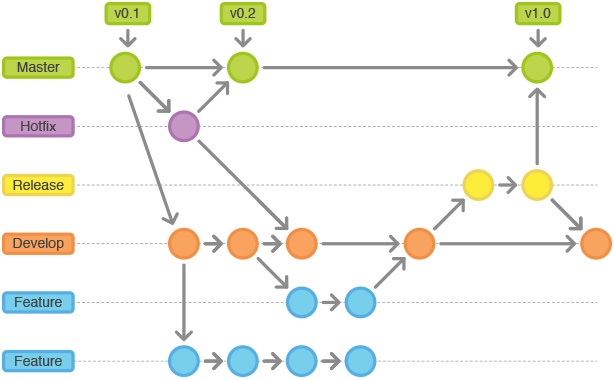
\includegraphics[scale=0.6]{./graphics/git_workflow} \\~\\
 \textbf{\textit{Figure 5: Workflow mis en place pour le développement}}
\end{center}

\underline{Les branches principales, fixes et immuables :}

\textbf{Master} est la branche où tout est stable. Chaque commit correspond à une version stable du projet (release) qui peut être déployée en production 
et taguée en conséquence (vX.Y.Z).

\textbf{Develop} est la branche sur laquelle s’effectue le développement proprement dit. On y prépare les changements en vue de la prochaine release dans 
master. \\

\underline{Les branches secondaires qui se font et se défont avec le temps :}

\textbf{Feature} part de develop et se merge dans develop.
On crée une branche feature/xxx lorsque l’on travaille sur une fonctionnalité en particulier. Lorsqu’elle est terminée, on la merge dans develop 
pour ajouter la feature stable dans le scope de la prochaine release.

\textbf{Release} part de develop et se merge dans master et develop.
On crée une branche release/xxx à partir de develop lorsque celle-ci reflète l’état désiré de la release (l’ensemble des fonctionnalités du scope 
ont été mergées). Ainsi, on peut préparer la prochaine release tranquillement, corriger d’éventuels bugs et poursuivre le développement en parallèle. 
Une fois que la release est prête (stable) on merge alors la branche dans master, mais aussi dans develop pour mettre à jour les modifications apportées.

\textbf{Hotfix} part de master et se merge dans master et develop / release.
On crée une branche hotfix/xxx lorsque l’on veut résoudre un bug critique en production rapidement. C’est un peu comme une release non planifiée. 
Lorsque le correctif est développé, on le merge dans master avec le numéro de version qui convient, ainsi que dans develop (ou la branche release en 
cours, le cas échéant) pour mettre à jour les modifications apportées. \\
\newpage
Les bonnes pratiques:
\begin{itemize}
   \item Une feature = une partie bien spécifique du code;
   \item Une feature = une branche;
   \item Spliter des changements en petites étapes = commit;
   \item Commiter le plus souvent possible;
   \item Faire une review du code avant commit
\end{itemize} ~\\

\`{A} ne pas faire:
\begin{itemize}
   \item Developper sur la branche master
   \item Developper sur la branche de developpement
   \item Faire un rebase sur une branche impliquant plusieurs développeurs
   \item Supprimer des branches non mergées
   \item Utiliser git rebase interactive sur des commit déjà poussés sur le dêpot central
\end{itemize}

%---------------------------------------------------------------------------------------------------------------------------------------------
\section{\underline{Revue et points clef}}

Voir en section 2 les points 2.1, 2.2, 2.4 et 2.5, ainsi que le planing général en annexe.
%---------------------------------------------------------------------------------------------------------------------------------------------
\section{\underline{Procédure de suivi et d'avancement}}

La mélée quotidienne durera environ quinze minutes et chaque membre devra s'exprimer sur trois points:
\begin{itemize}
 \item Ce qu'il a fait la veille;
 \item Ce qu'il prévoit de faire aujourd'hui;
 \item Ses problèmes, blocages ou remarques.
\end{itemize}


Un fichier excel sera créer par le suivre l'avancement du sprint. Il listera toute les taches à réaliser, à qui elles sont attribués, les date de début 
et de fin prévue et un statut.

Un fichier excel sera créer pour suivre les différentes actions prévues à l'issue des réunions.

\newpage
%---------------------------------------------------------------------------------------------------------------------------------------------
\section{\underline{Annexes}}
\subsection{Planing général}
\begin{center}
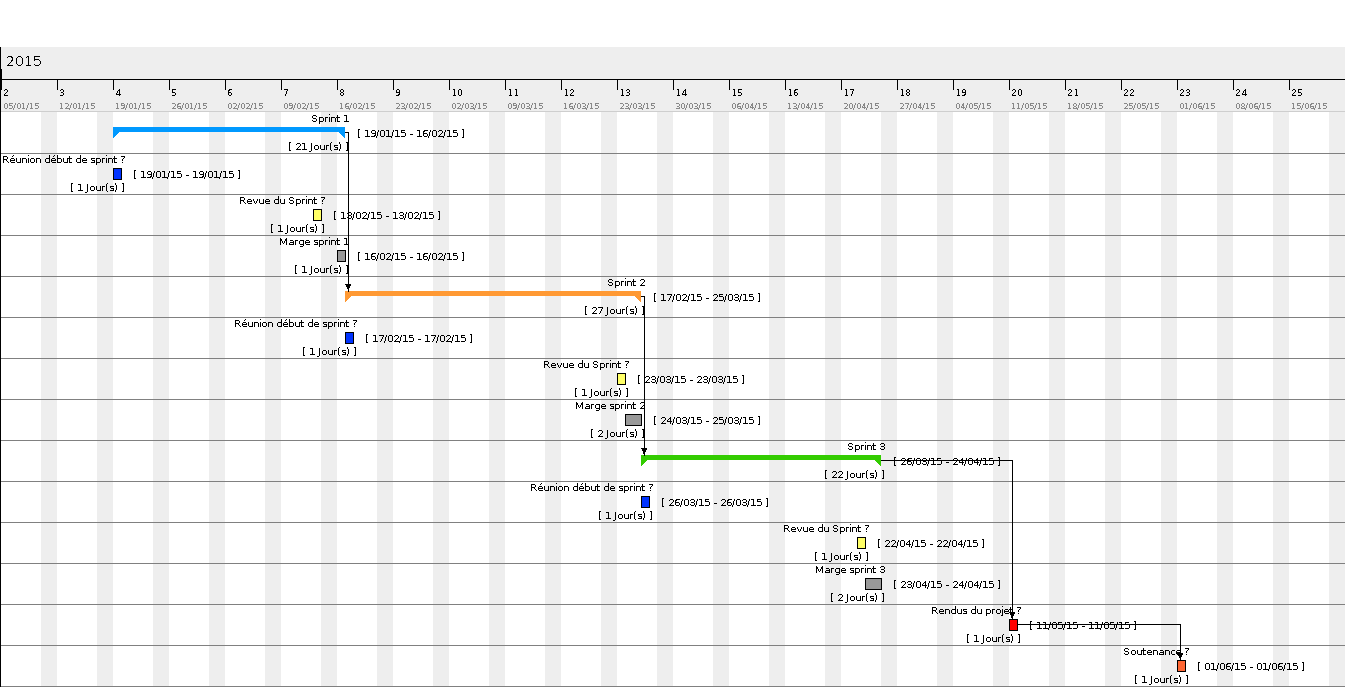
\includegraphics[angle=90,scale=0.63]{./graphics/Planing_general} \\~\\
\textbf{\textit{Figure 6: Planing général}}
\end{center}

\newpage
\subsection{Planing du sprint 1}
\begin{center}
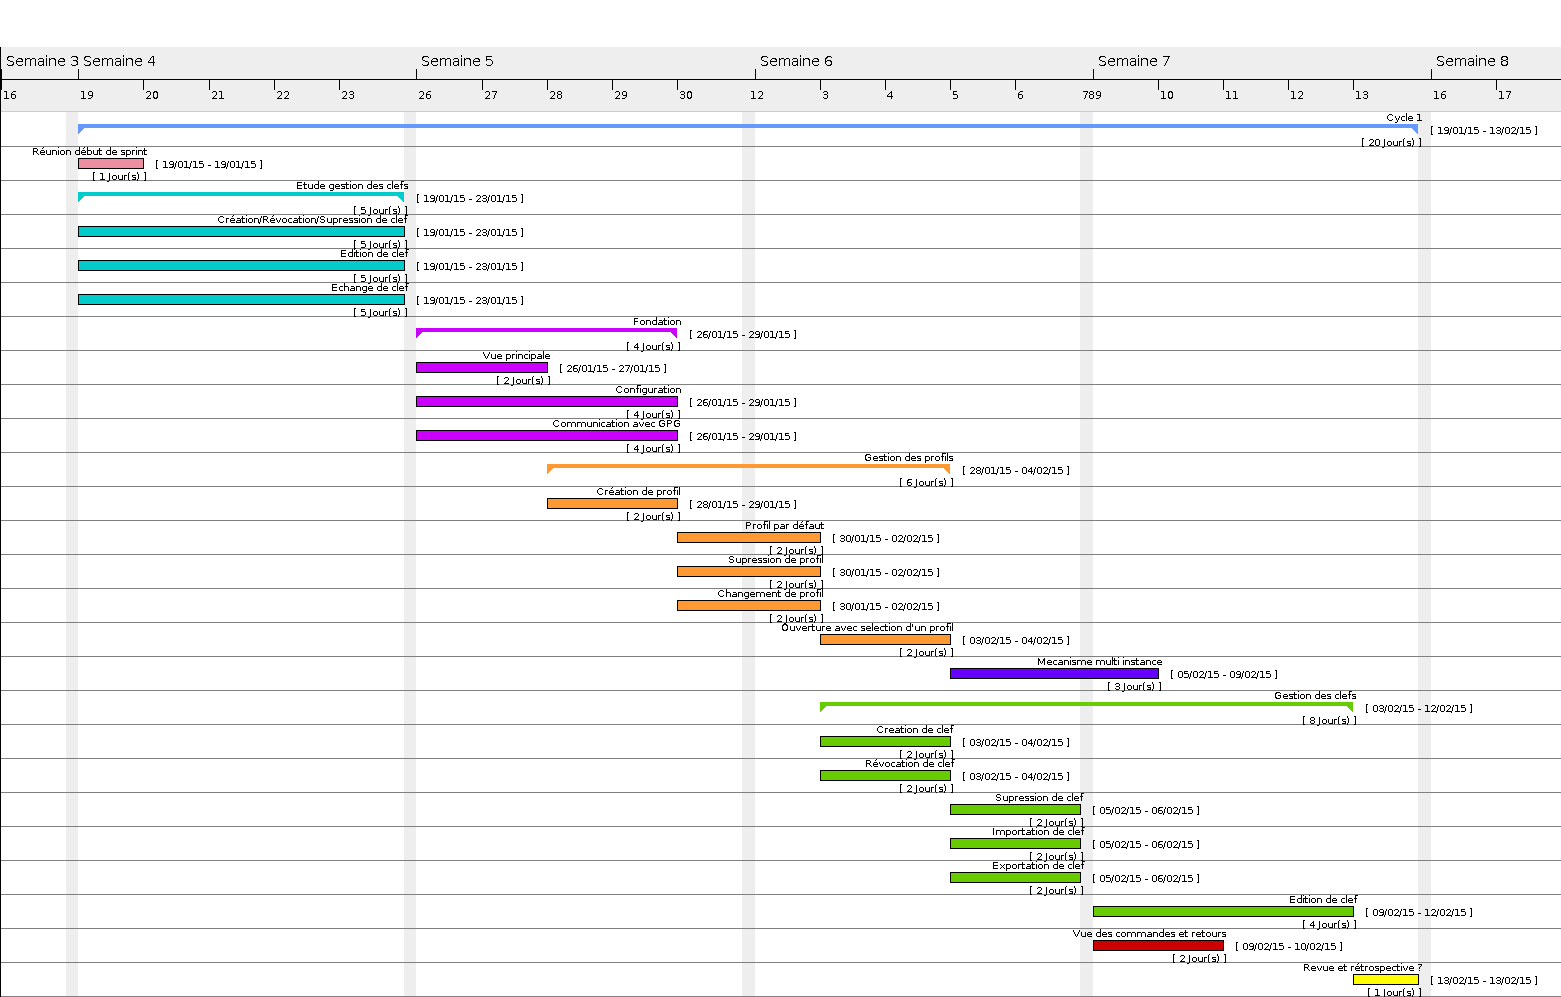
\includegraphics[angle=90,scale=0.385]{./graphics/Planing_sprint_1} \\~\\
\textbf{\textit{Figure 7: Planing du sprint 1 (1j/h = 1h30)}}
\end{center}
\end{document}

